\documentclass[a4paper,12pt]{article}

% Fonts {{{1
\usepackage{fontspec,amsmath,unicode-math}
\defaultfontfeatures{Ligatures=TeX}
\setmainfont[
  Path={/Users/yongrenjie/Library/Fonts/},
  Extension=.otf,
  UprightFont={*-regular},
  BoldFont={*-semibold},
  ItalicFont={*-italic},
  BoldItalicFont={*-semibolditalic},
]{minion3}
\setmonofont[
  Path={/Users/yongrenjie/Library/Fonts/},
  Extension=.otf,
  UprightFont={*-Regular},
  BoldFont={*-Bold},
  Scale=MatchLowercase
]{Inconsolata}
\setmathfont[
  Path={/Users/yongrenjie/Library/Fonts/},
  Scale=MatchLowercase
]{LibertinusMath-Regular.otf}
% Other optical sizes for Minion
\newfontfamily{\fontcaption}{minion3caption}[
  Path={/Users/yongrenjie/Library/Fonts/},
  Extension=.otf,
  UprightFont={*-regular},
  BoldFont={*-semibold},
  ItalicFont={*-italic},
  BoldItalicFont={*-semibolditalic},
]
\newfontfamily{\fontsubhead}{minion3subhead}[
  Path={/Users/yongrenjie/Library/Fonts/},
  Extension=.otf,
  UprightFont={*-regular},
  BoldFont={*-bold},
  ItalicFont={*-italic},
  BoldItalicFont={*-bolditalic},
]
\usepackage[final]{microtype}
% }}}1
% Packages and settings {{{1
\usepackage[font=small,labelfont=it,margin=15pt]{caption}
\usepackage{fullpage,parskip,graphicx,float,braket,setspace,subcaption}
\usepackage[svgnames]{xcolor}
\usepackage{chemformula}
\setchemformula{math-scripts=true}
\usepackage[style=chem-acs,subentry,articletitle,doi]{biblatex}
\addbibresource{abbs.bib}
\graphicspath{{./figures/}}
\usepackage{xurl}   % must be after biblatex
\usepackage[
  mode=match,
  range-phrase={--},
  range-units=single,
  propagate-math-font=true,
  reset-math-version=false,
  reset-text-family=false,
  reset-text-series=false,
  text-family-to-math=true,
  text-series-to-math=true
]{siunitx}
\usepackage[symbol]{footmisc}
\usepackage{titletoc}
\usepackage{hyperref}
\hypersetup{
    naturalnames,
    colorlinks,
    linkcolor={red!50!black},
    citecolor={blue!60!black},
    urlcolor={blue!80!black}
}
\usepackage[capitalise,noabbrev]{cleveref}

\usepackage{usebib}
\newbibfield{entryset}
\bibinput{abbs}

\onehalfspacing
\DeclareSIUnit{\molar}{\textsc{m}}
\DeclareSIUnit{\ppm}{ppm}
% }}}1
% Newcommands {{{1 
\newcommand{\articletitle}{Article Title Goes Here}
\newcommand{\crl}{Chemistry Research Laboratory, Department of Chemistry, University of Oxford, Mansfield Road, Oxford, OX1 3TA, United Kingdom}
\newcommand{\brukeruk}{Bruker UK Ltd, R\&D, Coventry CV4 9GH, United Kingdom}
\newcommand{\proton}{\ch{^{1}H}}
\newcommand{\carbonbulk}{\ch{^{12}C}}
\newcommand{\carbon}{\ch{^{13}C}}
\newcommand{\nitrogen}{\ch{^{15}N}}
\newcommand{\CH}{\carbon{}--\proton{}}
\newcommand{\HC}{\proton{}--\carbon{}}
\newcommand{\NH}{\nitrogen{}--\proton{}}
\newcommand{\HN}{\proton{}--\nitrogen{}}
\newcommand{\HH}{\proton{}--\proton{}}
\newcommand{\magn}[1]{\ch{^1H}$^{#1}$}
\newcommand{\magnnot}[1]{\ch{^1H}$^{!#1}$}
\newcommand{\todo}[1]{{\color{OrangeRed}#1}}
\newcommand{\autociteset}[1]{\autocite{\usebibentry{#1}{entryset}}}
\newcommand{\onejch}{{}^1\!J_{\ch{CH}}}
\newcommand{\onejcc}{{}^1\!J_{\ch{CC}}}
\newcommand{\onejnh}{{}^1\!J_{\ch{NH}}}
\newcommand{\onejxh}{{}^1\!J_{\ch{XH}}}
\newcommand{\njch}{{}^n\!J_{\ch{CH}}}
\newcommand{\njcc}{{}^n\!J_{\ch{CC}}}
\newcommand{\njnh}{{}^n\!J_{\ch{NH}}}
\newcommand{\theurl}{\url{https://nmr-genesis.co.uk}}
\newcommand*{\brucine}{Spectra were obtained on a \SI{700}{\MHz} Bruker AV III equipped with a TCI H/C/N cryoprobe; the sample used was \SI{50}{\milli\molar} brucine in \ch{CDCl3}.}
\newcommand*{\grami}{Spectra were obtained on a \SI{700}{\MHz} Bruker AV III equipped with a TCI H/C/N cryoprobe; the sample used was \SI{40}{\milli\molar} gramicidin in DMSO-\(d_6\).}
\newcommand*{\cyclo}{Spectra were obtained on a \SI{700}{\MHz} Bruker AV III equipped with a TCI H/C/N cryoprobe; the sample used was \SI{50}{\milli\molar} cyclosporin A in \ch{C6D6}.}
\newcommand*{\zolmi}{Spectra were obtained on a \SI{700}{\MHz} Bruker AV III equipped with a TCI H/C/N cryoprobe; the sample used was \SI{50}{\milli\molar} zolmitriptan in DMSO-\(d_6\).}
% }}}1
% NOAH newcommands {{{1
\newcommand*{\noahtwo}[2]{\csname noah#1\endcsname\csname noah#2\endcsname}
\newcommand*{\noahthree}[3]{\csname noah#1\endcsname\csname noah#2\endcsname\csname noah#3\endcsname}
\newcommand*{\noahfour}[4]{\csname noah#1\endcsname\csname noah#2\endcsname\csname noah#3\endcsname\csname noah#4\endcsname}
\newcommand*{\noahfive}[5]{\csname noah#1\endcsname\csname noah#2\endcsname\csname noah#3\endcsname\csname noah#4\endcsname\csname noah#5\endcsname}
\newcommand*{\noahA}{A}
\newcommand*{\noahB}{B}
\newcommand*{\noahBn}{B${}_{\ch{N}}$}
\newcommand*{\noahS}{S}
\newcommand*{\noahSp}{S${}^+$}
\newcommand*{\noahSpn}{S${}^+_{\ch{N}}$}
% }}}1

\begin{document}
\begin{refsection}

\begin{center}   % Front matter
    \textbf{\Large \articletitle{}}

    \vspace{0.2cm}

    Jonathan R.\ J.\ Yong,\textsuperscript{1} {\=E}riks Kup{\v{c}}e,\textsuperscript{2} Tim D. W. Claridge\textsuperscript{1,\texttt{*}}

    \vspace{0.2cm}

    \textsuperscript{1} \textit{\crl{}}

    \textsuperscript{2} \textit{\brukeruk{}}

    \textsuperscript{\texttt{*}} \texttt{tim.claridge@chem.ox.ac.uk}

    \vspace{0.5cm} \hrule

\end{center}

\section*{Abstract}

Yada yada...

\section{Introduction}

\todo{(Lightly paraphrased from GENESIS paper with more of a focus on structure elucidation... Let me know if I should shake it up a bit more.)}

Nuclear magnetic resonance (NMR) spectroscopy plays a key role in the structural elucidation of natural products.\autociteset{textbooks}
In particular, two-dimensional (2D) NMR experiments such as COSY, HSQC, HMBC, and NOESY provide vast amounts of information on through-bond and through-space molecular connectivity, allowing structures to be pieced together much like a jigsaw puzzle.
However, these experiments are often time-consuming as they require the incrementation of indirect-dimension evolution periods in order to construct the requisite 2D data matrices.
One particularly flexible method for accelerating 2D data acquisition is the NOAH (NMR by Ordered Acquisition using \proton{} detection) technique\autociteset{noah}, in which multiple 2D experiments (`modules') are combined into a single experiment using only a single recovery delay.
\todo{[Seems overkill to cite everything... perhaps just orig ACIE plus reviews?]}
These nested `supersequences', which rely on the tailored excitation of magnetisation from different sources, provide an array of 2D spectra (up to 10 so far) in greatly reduced experiment times.

Although virtually all common 2D experiments have been implemented in NOAH, these may fall short in proton-sparse molecules\autociteset{proton_sparse} which yield insufficient correlations.
In such cases, recourse must be made to other experiments which typically detect either long-range X--\proton{} couplings (as in the HMBC experiment\autociteset{n15_hmbc}, X = \carbon{} or \nitrogen{}), or \carbon{}--\carbon{} correlations (as in the INADEQUATE\autocite{Bax1981JACS}---or more practically, ADEQUATE\autociteset{adequate}---experiments).
Although these rely on heteronuclei (or pairs thereof) with low natural abundances, they allow chemists to directly trace out carbon- and nitrogen-containing backbones with much greater certainty.
Furthermore, with the introduction of cryogenically cooled probes and concomitant improvements in signal-to-noise ratio (SNR), such experiments can nowadays be feasibly run on dilute samples.

To date, insensitive experiments such as \nitrogen{} HMBC and ADEQUATE have not been incorporated into NOAH supersequences.
This is because in a traditional `linear' supersequence, each constituent module is recorded with the same number of transients.
The total experiment duration is therefore dictated by the module with the lowest sensitivity, and higher-sensitivity modules (e.g. HSQC or COSY) would be recorded with far more transients than would be necessary.
Although the more sensitive modules would still be obtained `for free', the effective time savings thus realised would be far smaller than for a supersequence with balanced sensitivities.
\todo{[this is actually best explained in RSC book chapter...]}

For this reason, the low-sensitivity ADEQUATE and \nitrogen{} HMBC modules form a `natural' pairing in a NOAH-2 \noahtwo{A}{Bn} supersequence, as will be shown in this work.
However, we also go beyond this to add more sensitive modules: not using   `horizontal' concatenation as in a traditional supersequence, but instead through `vertical' interleaving, analogously to the `parallel' supersequences recently described.\autocite{Kupce2021JACSA}
This approach, which effectively amounts to modifying the number of transients for each module, provides a powerful and flexible way to balance modules with different sensitivities.
We show that up to four modules (\nitrogen{} HMBC, \carbon{} HMBC, \nitrogen{} seHSQC, and \carbon{} HSQC) may be interleaved in this fashion, thereby fully generalising our previous work on parallel supersequences, where only two modules were interleaved at a time.

\todo{
    A mildly interesting question would be whether the resulting spectra can be processed -- using covariance techniques for example --- to yield \carbon{}-\nitrogen{} correlation spectra... Some references:

    \begin{itemize}
        \item \texttt{10.1002/mrc.1947}
        \item \texttt{10.1002/jhet.5570440541}
        \item \texttt{10.1002/mrc.2029}
        \item HSQC + ADEQUATE to get what's effectively a \carbon{}-\carbon{} COSY: \texttt{10.1002/mrc.2743}
    \end{itemize}

    Another obvious question would be whether the $1,1$-ADEQUATE which we've exclusively used here can be replaced with $1,n$-ADEQUATE; it may be useful to preemptively mention a yes or no in the text...
}

\begin{figure}[ht]
    \centering
    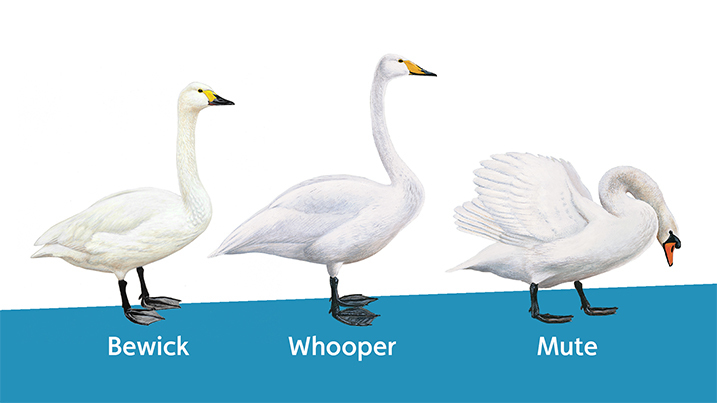
\includegraphics[width=0.8\textwidth]{swans.jpeg}
    {\phantomsubcaption\label{fig:swans_bewick}}
    {\phantomsubcaption\label{fig:swans_whooper}}
    {\phantomsubcaption\label{fig:swans_mute}}
    \caption{
        An array of adorable swans found in the United Kingdom.
        \textbf{(\subref{fig:swans_bewick})} Bewick's swan (\textit{Cygnus columbianus bewickii}).
        \textbf{(\subref{fig:swans_whooper})} Whooper swan (\textit{Cygnus cygnus}).
        \textbf{(\subref{fig:swans_mute})} Mute swan (\textit{Cygnus olor}).
        (Picture credit: Wildfowl and Wetlands Trust.)
    }
    \label{fig:swans}
\end{figure}

\section{NOAH-2 AB\texorpdfstring{$_{\ch{N}}$}{n}}

ADEQUATE first -- lowest sensitivity

must preserve \magnnot{\ch{C}} magnetisation, thus use ZIP in the ADEQUATE module\autocite{Hansen2021AC, Yong2021JMR} \todo{(similar to BANGO, give them a shoutout ...... why do I even bother being kind)}

\nitrogen{} HMBC: QF mode simplest and found to work best

show data on brucine

SNR comparison

\section{NOAH-3 AB\texorpdfstring{$_{\ch{N}}$}{n}B\texorpdfstring{$_{\ch{N}}$}{n}}

$\njnh{}$ tends to vary -- variety of ways to get around this such as accordion-type experiments typified by IMPEACH-MBC\autociteset{accordion_hmbc}

other citations, ACCORD-HMBC, CIGAR-HMBC

\section{NOAH-4 AB\texorpdfstring{$_{\ch{N}}$}{n}BS}

\section{NOAH-5 AB\texorpdfstring{$_{\ch{N}}$}{n}BS\texorpdfstring{$^+_{\ch{N}}$}{+n}S}

Cyclosporine

\section{Conclusion}

\section*{Acknowledgements}

We thank Dr Mohammadali Foroozandeh (University of Oxford) for helpful discussions.
J.R.J.Y.\ thanks the Clarendon Fund (University of Oxford) and the EPSRC Centre for Doctoral Training in Synthesis for Biology and Medicine (EP/L015838/1) for a studentship, generously supported by AstraZeneca, Diamond Light Source, Defence Science and Technology Laboratory, Evotec, GlaxoSmithKline, Janssen, Novartis, Pfizer, Syngenta, Takeda, UCB, and Vertex.

% Fakesection Bibliography
\AtNextBibliography{\small}
\printbibliography{}
\end{refsection}


% Fakesection ================= SI ==================

\clearpage
\begin{refsection}
\newcommand{\sectionbreak}{\clearpage}
\renewcommand*{\thefigure}{S\arabic{figure}}
\renewcommand*{\thesection}{S\arabic{section}}
\renewcommand*{\thetable}{S\arabic{table}}
\renewcommand*{\thepage}{S\arabic{page}}
\setcounter{page}{1}
\setcounter{figure}{0}
\setcounter{section}{0}
\setcounter{table}{0}
\onehalfspacing

\hspace{0pt}
\vfill
\begin{center}
    \huge
    Supporting Information

    \vspace{0.3cm}

    \textit{for}

    \vspace{0.3cm}

    \articletitle{}

    \vspace{0.6cm}

    \Large Jonathan R.\ J.\ Yong,\textsuperscript{1} {\=E}riks Kup{\v{c}}e,\textsuperscript{2} Tim D.\ W.\ Claridge\textsuperscript{1,\texttt{*}}

    \vspace{0.6cm}

    \large \textsuperscript{1} \textit{\crl{}}

    \textsuperscript{2} \textit{\brukeruk{}}

    \textsuperscript{\texttt{*}} \texttt{tim.claridge@chem.ox.ac.uk}

\end{center}

\vspace{2cm}
\section*{Contents}

\startcontents[si]
\printcontents[si]{ }{1}{}
\vfill
\hspace{0pt}
\newpage

\section{Pulse programme setup}

It's complicated as all hell, GENESIS\autocite{Yong2022AC} doesn't do it either (and for good reason).

% Fakesection SI bibliography
\AtNextBibliography{\small}
\printbibliography{}
\clearpage    % For some reason this is needed to make the last page number 'S5', not '5'

\end{refsection}

\end{document}
